\documentclass[1p]{elsarticle_modified}
%\bibliographystyle{elsarticle-num}

%\usepackage[colorlinks]{hyperref}
%\usepackage{abbrmath_seonhwa} %\Abb, \Ascr, \Acal ,\Abf, \Afrak
\usepackage{amsfonts}
\usepackage{amssymb}
\usepackage{amsmath}
\usepackage{amsthm}
\usepackage{scalefnt}
\usepackage{amsbsy}
\usepackage{kotex}
\usepackage{caption}
\usepackage{subfig}
\usepackage{color}
\usepackage{graphicx}
\usepackage{xcolor} %% white, black, red, green, blue, cyan, magenta, yellow
\usepackage{float}
\usepackage{setspace}
\usepackage{hyperref}

\usepackage{tikz}
\usetikzlibrary{arrows}

\usepackage{multirow}
\usepackage{array} % fixed length table
\usepackage{hhline}

%%%%%%%%%%%%%%%%%%%%%
\makeatletter
\renewcommand*\env@matrix[1][\arraystretch]{%
	\edef\arraystretch{#1}%
	\hskip -\arraycolsep
	\let\@ifnextchar\new@ifnextchar
	\array{*\c@MaxMatrixCols c}}
\makeatother %https://tex.stackexchange.com/questions/14071/how-can-i-increase-the-line-spacing-in-a-matrix
%%%%%%%%%%%%%%%

\usepackage[normalem]{ulem}

\newcommand{\msout}[1]{\ifmmode\text{\sout{\ensuremath{#1}}}\else\sout{#1}\fi}
%SOURCE: \msout is \stkout macro in https://tex.stackexchange.com/questions/20609/strikeout-in-math-mode

\newcommand{\cancel}[1]{
	\ifmmode
	{\color{red}\msout{#1}}
	\else
	{\color{red}\sout{#1}}
	\fi
}

\newcommand{\add}[1]{
	{\color{blue}\uwave{#1}}
}

\newcommand{\replace}[2]{
	\ifmmode
	{\color{red}\msout{#1}}{\color{blue}\uwave{#2}}
	\else
	{\color{red}\sout{#1}}{\color{blue}\uwave{#2}}
	\fi
}

\newcommand{\Sol}{\mathcal{S}} %segment
\newcommand{\D}{D} %diagram
\newcommand{\A}{\mathcal{A}} %arc


%%%%%%%%%%%%%%%%%%%%%%%%%%%%%5 test

\def\sl{\operatorname{\textup{SL}}(2,\Cbb)}
\def\psl{\operatorname{\textup{PSL}}(2,\Cbb)}
\def\quan{\mkern 1mu \triangleright \mkern 1mu}

\theoremstyle{definition}
\newtheorem{thm}{Theorem}[section]
\newtheorem{prop}[thm]{Proposition}
\newtheorem{lem}[thm]{Lemma}
\newtheorem{ques}[thm]{Question}
\newtheorem{cor}[thm]{Corollary}
\newtheorem{defn}[thm]{Definition}
\newtheorem{exam}[thm]{Example}
\newtheorem{rmk}[thm]{Remark}
\newtheorem{alg}[thm]{Algorithm}

\newcommand{\I}{\sqrt{-1}}
\begin{document}

%\begin{frontmatter}
%
%\title{Boundary parabolic representations of knots up to 8 crossings}
%
%%% Group authors per affiliation:
%\author{Yunhi Cho} 
%\address{Department of Mathematics, University of Seoul, Seoul, Korea}
%\ead{yhcho@uos.ac.kr}
%
%
%\author{Seonhwa Kim} %\fnref{s_kim}}
%\address{Center for Geometry and Physics, Institute for Basic Science, Pohang, 37673, Korea}
%\ead{ryeona17@ibs.re.kr}
%
%\author{Hyuk Kim}
%\address{Department of Mathematical Sciences, Seoul National University, Seoul 08826, Korea}
%\ead{hyukkim@snu.ac.kr}
%
%\author{Seokbeom Yoon}
%\address{Department of Mathematical Sciences, Seoul National University, Seoul, 08826,  Korea}
%\ead{sbyoon15@snu.ac.kr}
%
%\begin{abstract}
%We find all boundary parabolic representation of knots up to 8 crossings.
%
%\end{abstract}
%\begin{keyword}
%    \MSC[2010] 57M25 
%\end{keyword}
%
%\end{frontmatter}

%\linenumbers
%\tableofcontents
%
\newcommand\colored[1]{\textcolor{white}{\rule[-0.35ex]{0.8em}{1.4ex}}\kern-0.8em\color{red} #1}%
%\newcommand\colored[1]{\textcolor{white}{ #1}\kern-2.17ex	\textcolor{white}{ #1}\kern-1.81ex	\textcolor{white}{ #1}\kern-2.15ex\color{red}#1	}

{\Large $\underline{12a_{0465}~(K12a_{0465})}$}

\setlength{\tabcolsep}{10pt}
\renewcommand{\arraystretch}{1.6}
\vspace{1cm}\begin{tabular}{m{100pt}>{\centering\arraybackslash}m{274pt}}
\multirow{5}{120pt}{
	\centering
	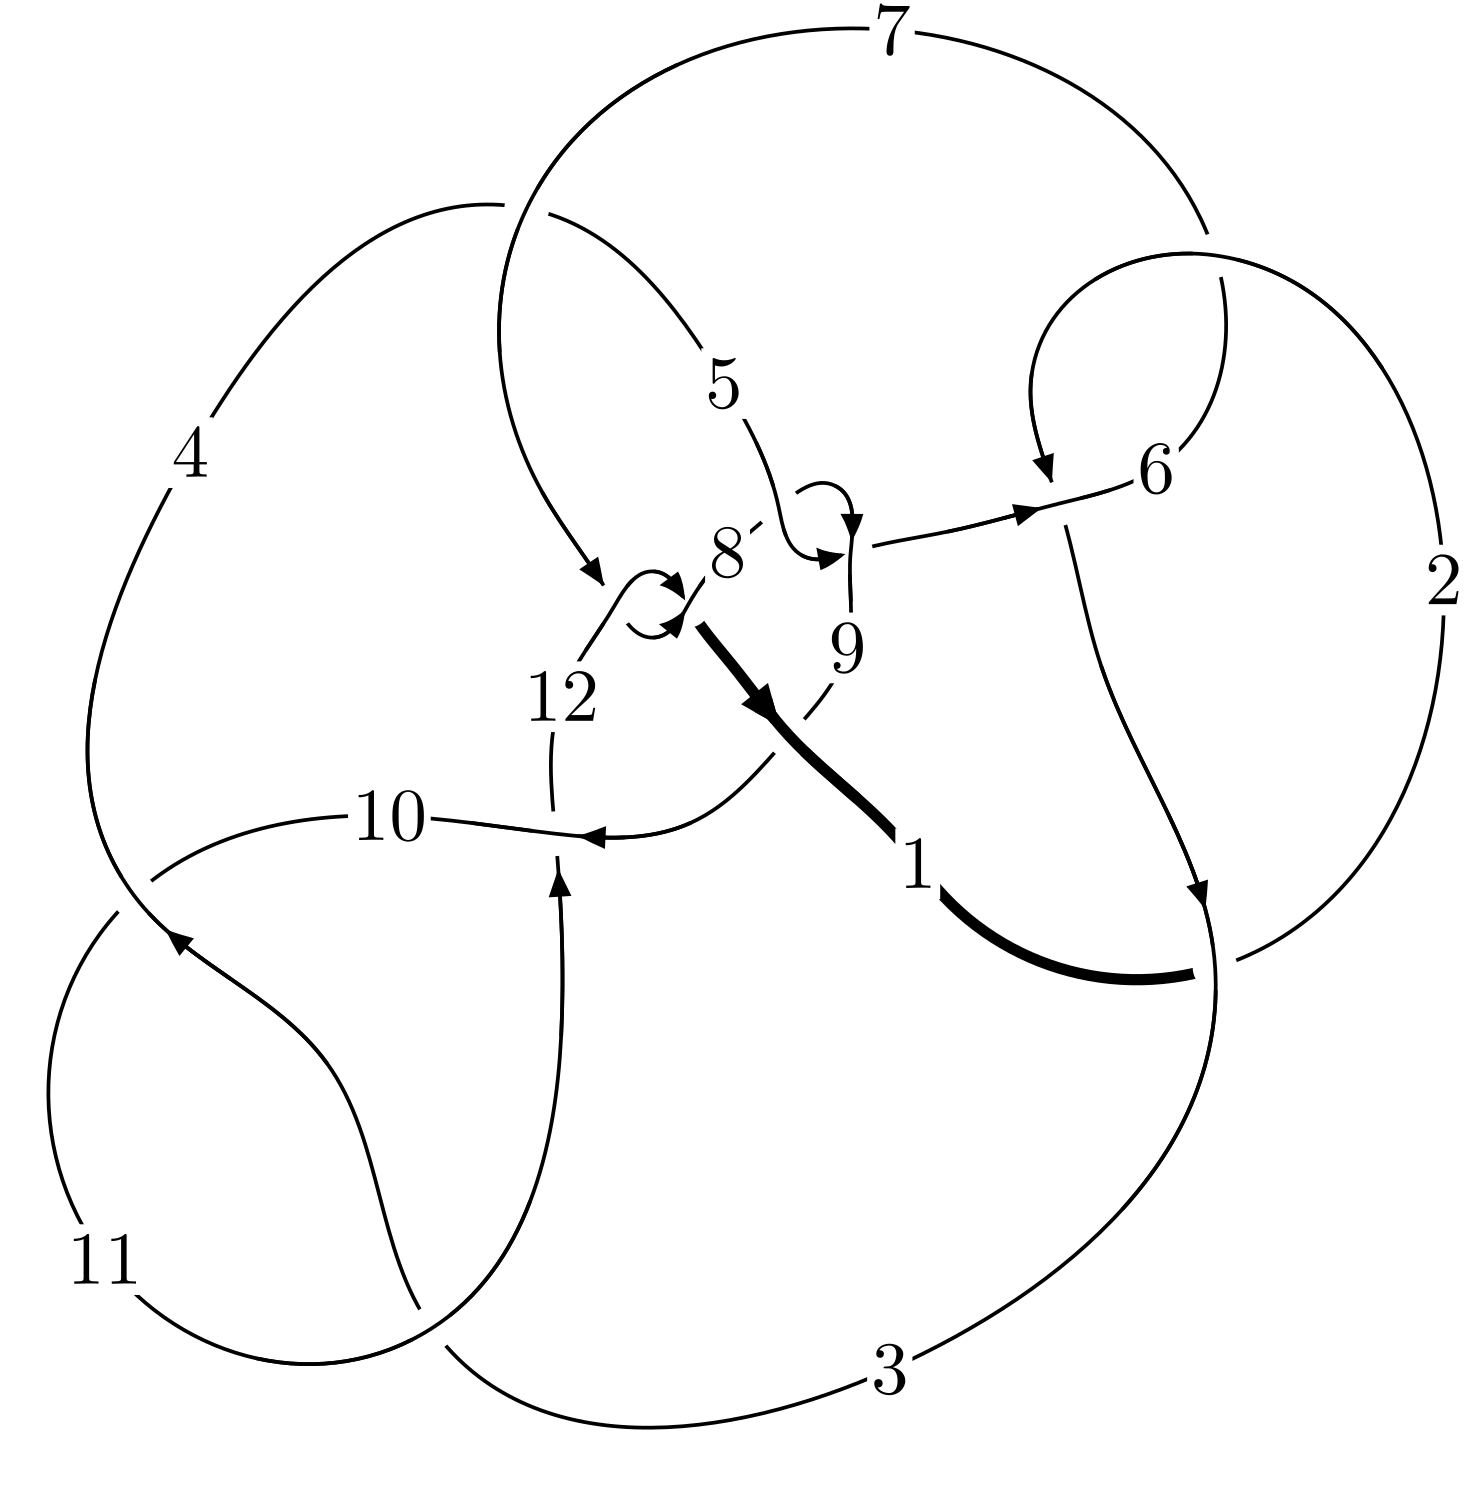
\includegraphics[width=112pt]{../../../GIT/diagram.site/Diagrams/png/1266_12a_0465.png}\\
\ \ \ A knot diagram\footnotemark}&
\allowdisplaybreaks
\textbf{Linearized knot diagam} \\
\cline{2-2}
 &
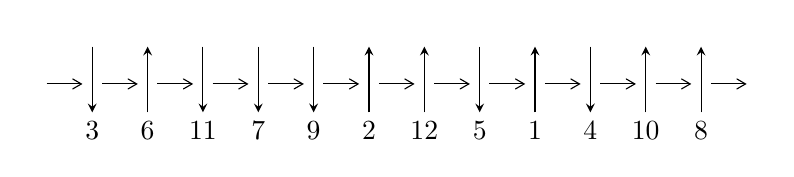
\begin{tikzpicture}[x=20pt, y=17pt]
	% nodes
	\node (C0) at (0, 0) {};
	\node (C1) at (1, 0) {};
	\node (C1U) at (1, +1) {};
	\node (C1D) at (1, -1) {3};

	\node (C2) at (2, 0) {};
	\node (C2U) at (2, +1) {};
	\node (C2D) at (2, -1) {6};

	\node (C3) at (3, 0) {};
	\node (C3U) at (3, +1) {};
	\node (C3D) at (3, -1) {11};

	\node (C4) at (4, 0) {};
	\node (C4U) at (4, +1) {};
	\node (C4D) at (4, -1) {7};

	\node (C5) at (5, 0) {};
	\node (C5U) at (5, +1) {};
	\node (C5D) at (5, -1) {9};

	\node (C6) at (6, 0) {};
	\node (C6U) at (6, +1) {};
	\node (C6D) at (6, -1) {2};

	\node (C7) at (7, 0) {};
	\node (C7U) at (7, +1) {};
	\node (C7D) at (7, -1) {12};

	\node (C8) at (8, 0) {};
	\node (C8U) at (8, +1) {};
	\node (C8D) at (8, -1) {5};

	\node (C9) at (9, 0) {};
	\node (C9U) at (9, +1) {};
	\node (C9D) at (9, -1) {1};

	\node (C10) at (10, 0) {};
	\node (C10U) at (10, +1) {};
	\node (C10D) at (10, -1) {4};

	\node (C11) at (11, 0) {};
	\node (C11U) at (11, +1) {};
	\node (C11D) at (11, -1) {10};

	\node (C12) at (12, 0) {};
	\node (C12U) at (12, +1) {};
	\node (C12D) at (12, -1) {8};
	\node (C13) at (13, 0) {};

	% arrows
	\draw[->,>={angle 60}]
	(C0) edge (C1) (C1) edge (C2) (C2) edge (C3) (C3) edge (C4) (C4) edge (C5) (C5) edge (C6) (C6) edge (C7) (C7) edge (C8) (C8) edge (C9) (C9) edge (C10) (C10) edge (C11) (C11) edge (C12) (C12) edge (C13) ;	\draw[->,>=stealth]
	(C1U) edge (C1D) (C2D) edge (C2U) (C3U) edge (C3D) (C4U) edge (C4D) (C5U) edge (C5D) (C6D) edge (C6U) (C7D) edge (C7U) (C8U) edge (C8D) (C9D) edge (C9U) (C10U) edge (C10D) (C11D) edge (C11U) (C12D) edge (C12U) ;
	\end{tikzpicture} \\
\hhline{~~} \\& 
\textbf{Solving Sequence} \\ \cline{2-2} 
 &
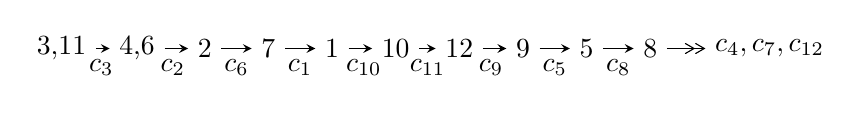
\begin{tikzpicture}[x=23pt, y=7pt]
	% node
	\node (A0) at (-1/8, 0) {3,11};
	\node (A1) at (17/16, 0) {4,6};
	\node (A2) at (17/8, 0) {2};
	\node (A3) at (25/8, 0) {7};
	\node (A4) at (33/8, 0) {1};
	\node (A5) at (41/8, 0) {10};
	\node (A6) at (49/8, 0) {12};
	\node (A7) at (57/8, 0) {9};
	\node (A8) at (65/8, 0) {5};
	\node (A9) at (73/8, 0) {8};
	\node (C1) at (1/2, -1) {$c_{3}$};
	\node (C2) at (13/8, -1) {$c_{2}$};
	\node (C3) at (21/8, -1) {$c_{6}$};
	\node (C4) at (29/8, -1) {$c_{1}$};
	\node (C5) at (37/8, -1) {$c_{10}$};
	\node (C6) at (45/8, -1) {$c_{11}$};
	\node (C7) at (53/8, -1) {$c_{9}$};
	\node (C8) at (61/8, -1) {$c_{5}$};
	\node (C9) at (69/8, -1) {$c_{8}$};
	\node (A10) at (11, 0) {$c_{4},c_{7},c_{12}$};

	% edge
	\draw[->,>=stealth]	
	(A0) edge (A1) (A1) edge (A2) (A2) edge (A3) (A3) edge (A4) (A4) edge (A5) (A5) edge (A6) (A6) edge (A7) (A7) edge (A8) (A8) edge (A9) ;
	\draw[->>,>={angle 60}]	
	(A9) edge (A10);
\end{tikzpicture} \\ 

\end{tabular} \\

\footnotetext{
The image of knot diagram is generated by the software ``\textbf{Draw programme}" developed by Andrew Bartholomew(\url{http://www.layer8.co.uk/maths/draw/index.htm\#Running-draw}), where we modified some parts for our purpose(\url{https://github.com/CATsTAILs/LinksPainter}).
}\phantom \\ \newline 
\centering \textbf{Ideals for irreducible components\footnotemark of $X_{\text{par}}$} 
 
\begin{align*}
I^u_{1}&=\langle 
1.94916\times10^{307} u^{131}-3.65279\times10^{307} u^{130}+\cdots+2.01785\times10^{308} b-1.09127\times10^{309},\\
\phantom{I^u_{1}}&\phantom{= \langle  }-3.70110\times10^{309} u^{131}+8.38178\times10^{309} u^{130}+\cdots+2.68374\times10^{310} a+3.35444\times10^{311},\\
\phantom{I^u_{1}}&\phantom{= \langle  }u^{132}-2 u^{131}+\cdots-476 u+76\rangle \\
I^u_{2}&=\langle 
3 a u+9 b+12 a+5 u+11,\;18 a^2+3 a u+48 a+u+37,\;u^2+2\rangle \\
I^u_{3}&=\langle 
-9 a u+7 b+3 a+2 u-3,\;9 a^2-6 a u-5 u-11,\;u^2- u+1\rangle \\
I^u_{4}&=\langle 
b,\;a+u,\;u^2+u+1\rangle \\
\\
I^v_{1}&=\langle 
a,\;b+v,\;v^2- v+1\rangle \\
\end{align*}
\raggedright * 5 irreducible components of $\dim_{\mathbb{C}}=0$, with total 144 representations.\\
\footnotetext{All coefficients of polynomials are rational numbers. But the coefficients are sometimes approximated in decimal forms when there is not enough margin.}
\newpage
\renewcommand{\arraystretch}{1}
\centering \section*{I. $I^u_{1}= \langle 1.95\times10^{307} u^{131}-3.65\times10^{307} u^{130}+\cdots+2.02\times10^{308} b-1.09\times10^{309},\;-3.70\times10^{309} u^{131}+8.38\times10^{309} u^{130}+\cdots+2.68\times10^{310} a+3.35\times10^{311},\;u^{132}-2 u^{131}+\cdots-476 u+76 \rangle$}
\flushleft \textbf{(i) Arc colorings}\\
\begin{tabular}{m{7pt} m{180pt} m{7pt} m{180pt} }
\flushright $a_{3}=$&$\begin{pmatrix}1\\0\end{pmatrix}$ \\
\flushright $a_{11}=$&$\begin{pmatrix}0\\u\end{pmatrix}$ \\
\flushright $a_{4}=$&$\begin{pmatrix}1\\u^2\end{pmatrix}$ \\
\flushright $a_{6}=$&$\begin{pmatrix}0.137909 u^{131}-0.312317 u^{130}+\cdots+84.5087 u-12.4991\\-0.0965960 u^{131}+0.181024 u^{130}+\cdots-30.2730 u+5.40808\end{pmatrix}$ \\
\flushright $a_{2}=$&$\begin{pmatrix}0.199343 u^{131}-0.396256 u^{130}+\cdots+127.923 u-23.4017\\-0.0527294 u^{131}+0.131771 u^{130}+\cdots-4.97262 u-1.02232\end{pmatrix}$ \\
\flushright $a_{7}=$&$\begin{pmatrix}0.112731 u^{131}-0.391881 u^{130}+\cdots+143.590 u-27.1262\\-0.0759172 u^{131}+0.171870 u^{130}+\cdots-15.7531 u+0.451833\end{pmatrix}$ \\
\flushright $a_{1}=$&$\begin{pmatrix}0.146613 u^{131}-0.264486 u^{130}+\cdots+122.951 u-24.4240\\-0.0527294 u^{131}+0.131771 u^{130}+\cdots-4.97262 u-1.02232\end{pmatrix}$ \\
\flushright $a_{10}=$&$\begin{pmatrix}u\\u^3+u\end{pmatrix}$ \\
\flushright $a_{12}=$&$\begin{pmatrix}u^3\\u^5+u^3+u\end{pmatrix}$ \\
\flushright $a_{9}=$&$\begin{pmatrix}0.0624762 u^{131}-0.0629818 u^{130}+\cdots+131.166 u-24.5816\\0.159767 u^{131}-0.280127 u^{130}+\cdots+76.3670 u-13.7238\end{pmatrix}$ \\
\flushright $a_{5}=$&$\begin{pmatrix}0.0225291 u^{131}-0.145369 u^{130}+\cdots-32.5467 u+5.91958\\-0.106550 u^{131}+0.113212 u^{130}+\cdots-20.2316 u+3.42718\end{pmatrix}$ \\
\flushright $a_{8}=$&$\begin{pmatrix}0.0687231 u^{131}-0.262340 u^{130}+\cdots+119.942 u-23.4880\\-0.0149219 u^{131}+0.0644011 u^{130}+\cdots+1.87048 u-1.24755\end{pmatrix}$\\&\end{tabular}
\flushleft \textbf{(ii) Obstruction class $= -1$}\\~\\
\flushleft \textbf{(iii) Cusp Shapes $= -0.497123 u^{131}+0.474012 u^{130}+\cdots-20.8223 u-10.5378$}\\~\\
\newpage\renewcommand{\arraystretch}{1}
\flushleft \textbf{(iv) u-Polynomials at the component}\newline \\
\begin{tabular}{m{50pt}|m{274pt}}
Crossings & \hspace{64pt}u-Polynomials at each crossing \\
\hline $$\begin{aligned}c_{1}\end{aligned}$$&$\begin{aligned}
&u^{132}+64 u^{131}+\cdots+14800 u+5776
\end{aligned}$\\
\hline $$\begin{aligned}c_{2},c_{6}\end{aligned}$$&$\begin{aligned}
&u^{132}-2 u^{131}+\cdots-476 u+76
\end{aligned}$\\
\hline $$\begin{aligned}c_{3},c_{10}\end{aligned}$$&$\begin{aligned}
&u^{132}+2 u^{131}+\cdots+476 u+76
\end{aligned}$\\
\hline $$\begin{aligned}c_{4}\end{aligned}$$&$\begin{aligned}
&2401(2401 u^{132}+37730 u^{131}+\cdots+8199247 u+3800453)
\end{aligned}$\\
\hline $$\begin{aligned}c_{5},c_{8}\end{aligned}$$&$\begin{aligned}
&u^{132}+3 u^{131}+\cdots+9208 u+1228
\end{aligned}$\\
\hline $$\begin{aligned}c_{7},c_{12}\end{aligned}$$&$\begin{aligned}
&u^{132}-3 u^{131}+\cdots-9208 u+1228
\end{aligned}$\\
\hline $$\begin{aligned}c_{9}\end{aligned}$$&$\begin{aligned}
&2401(2401 u^{132}-37730 u^{131}+\cdots-8199247 u+3800453)
\end{aligned}$\\
\hline $$\begin{aligned}c_{11}\end{aligned}$$&$\begin{aligned}
&u^{132}-64 u^{131}+\cdots-14800 u+5776
\end{aligned}$\\
\hline
\end{tabular}\\~\\
\newpage\renewcommand{\arraystretch}{1}
\flushleft \textbf{(v) Riley Polynomials at the component}\newline \\
\begin{tabular}{m{50pt}|m{274pt}}
Crossings & \hspace{64pt}Riley Polynomials at each crossing \\
\hline $$\begin{aligned}c_{1},c_{11}\end{aligned}$$&$\begin{aligned}
&y^{132}+16 y^{131}+\cdots+422881536 y+33362176
\end{aligned}$\\
\hline $$\begin{aligned}c_{2},c_{3},c_{6}\\c_{10}\end{aligned}$$&$\begin{aligned}
&y^{132}+64 y^{131}+\cdots+14800 y+5776
\end{aligned}$\\
\hline $$\begin{aligned}c_{4},c_{9}\end{aligned}$$&$\begin{aligned}
&5764801(5764801 y^{132}-1.97886\times10^{8} y^{131}+\cdots-2.94420\times10^{14} y+1.44434\times10^{13})
\end{aligned}$\\
\hline $$\begin{aligned}c_{5},c_{7},c_{8}\\c_{12}\end{aligned}$$&$\begin{aligned}
&y^{132}-65 y^{131}+\cdots-1106432 y+1507984
\end{aligned}$\\
\hline
\end{tabular}\\~\\
\newpage\flushleft \textbf{(vi) Complex Volumes and Cusp Shapes}
$$\begin{array}{c|c|c}  
\text{Solutions to }I^u_{1}& \I (\text{vol} + \sqrt{-1}CS) & \text{Cusp shape}\\
 \hline 
\begin{aligned}
u &= \phantom{-}0.823198 + 0.569211 I \\
a &= \phantom{-}0.889660 + 0.779506 I \\
b &= -0.190681 + 1.006910 I\end{aligned}
 & -1.53863 + 0.67688 I & \phantom{-0.000000 } 0 \\ \hline\begin{aligned}
u &= \phantom{-}0.823198 - 0.569211 I \\
a &= \phantom{-}0.889660 - 0.779506 I \\
b &= -0.190681 - 1.006910 I\end{aligned}
 & -1.53863 - 0.67688 I & \phantom{-0.000000 } 0 \\ \hline\begin{aligned}
u &= \phantom{-}0.559179 + 0.825258 I \\
a &= \phantom{-}4.50642 + 0.70465 I \\
b &= \phantom{-}0.440469 + 0.792376 I\end{aligned}
 & \phantom{-}0.105725 - 0.171371 I & \phantom{-0.000000 } 0 \\ \hline\begin{aligned}
u &= \phantom{-}0.559179 - 0.825258 I \\
a &= \phantom{-}4.50642 - 0.70465 I \\
b &= \phantom{-}0.440469 - 0.792376 I\end{aligned}
 & \phantom{-}0.105725 + 0.171371 I & \phantom{-0.000000 } 0 \\ \hline\begin{aligned}
u &= -0.424632 + 0.889847 I \\
a &= \phantom{-}1.42271 - 0.04850 I \\
b &= -0.03946 - 1.50799 I\end{aligned}
 & -5.98533 + 1.74123 I & \phantom{-0.000000 } 0 \\ \hline\begin{aligned}
u &= -0.424632 - 0.889847 I \\
a &= \phantom{-}1.42271 + 0.04850 I \\
b &= -0.03946 + 1.50799 I\end{aligned}
 & -5.98533 - 1.74123 I & \phantom{-0.000000 } 0 \\ \hline\begin{aligned}
u &= \phantom{-}0.936127 + 0.405809 I \\
a &= -0.808074 + 0.587728 I \\
b &= \phantom{-}0.624017 + 1.147650 I\end{aligned}
 & -2.30779 + 13.83220 I & \phantom{-0.000000 } 0 \\ \hline\begin{aligned}
u &= \phantom{-}0.936127 - 0.405809 I \\
a &= -0.808074 - 0.587728 I \\
b &= \phantom{-}0.624017 - 1.147650 I\end{aligned}
 & -2.30779 - 13.83220 I & \phantom{-0.000000 } 0 \\ \hline\begin{aligned}
u &= \phantom{-}0.305623 + 0.975415 I \\
a &= -2.36155 + 0.30402 I \\
b &= \phantom{-}0.725974 - 0.852806 I\end{aligned}
 & \phantom{-}3.22670 - 3.10282 I & \phantom{-0.000000 } 0 \\ \hline\begin{aligned}
u &= \phantom{-}0.305623 - 0.975415 I \\
a &= -2.36155 - 0.30402 I \\
b &= \phantom{-}0.725974 + 0.852806 I\end{aligned}
 & \phantom{-}3.22670 + 3.10282 I & \phantom{-0.000000 } 0\\
 \hline 
 \end{array}$$\newpage$$\begin{array}{c|c|c}  
\text{Solutions to }I^u_{1}& \I (\text{vol} + \sqrt{-1}CS) & \text{Cusp shape}\\
 \hline 
\begin{aligned}
u &= \phantom{-}0.190681 + 1.006910 I \\
a &= \phantom{-}1.87153 - 0.08400 I \\
b &= -0.823198 + 0.569211 I\end{aligned}
 & \phantom{-}1.53863 + 0.67688 I & \phantom{-0.000000 } 0 \\ \hline\begin{aligned}
u &= \phantom{-}0.190681 - 1.006910 I \\
a &= \phantom{-}1.87153 + 0.08400 I \\
b &= -0.823198 - 0.569211 I\end{aligned}
 & \phantom{-}1.53863 - 0.67688 I & \phantom{-0.000000 } 0 \\ \hline\begin{aligned}
u &= -0.065305 + 1.027270 I \\
a &= \phantom{-}1.121830 - 0.587024 I \\
b &= \phantom{-}0.065305 + 1.027270 I\end{aligned}
 & \phantom{-0.000000 -}3.95402 I & \phantom{-0.000000 } 0 \\ \hline\begin{aligned}
u &= -0.065305 - 1.027270 I \\
a &= \phantom{-}1.121830 + 0.587024 I \\
b &= \phantom{-}0.065305 - 1.027270 I\end{aligned}
 & \phantom{-0.000000 } -3.95402 I & \phantom{-0.000000 } 0 \\ \hline\begin{aligned}
u &= -0.840683 + 0.484130 I \\
a &= -0.764027 - 0.676827 I \\
b &= \phantom{-}0.312065 - 1.072640 I\end{aligned}
 & -5.44129 + 1.88998 I & \phantom{-0.000000 } 0 \\ \hline\begin{aligned}
u &= -0.840683 - 0.484130 I \\
a &= -0.764027 + 0.676827 I \\
b &= \phantom{-}0.312065 + 1.072640 I\end{aligned}
 & -5.44129 - 1.88998 I & \phantom{-0.000000 } 0 \\ \hline\begin{aligned}
u &= \phantom{-}0.780358 + 0.686992 I \\
a &= -0.500434 - 0.041443 I \\
b &= \phantom{-}0.615963 + 0.235511 I\end{aligned}
 & -1.84741 - 4.70427 I & \phantom{-0.000000 } 0 \\ \hline\begin{aligned}
u &= \phantom{-}0.780358 - 0.686992 I \\
a &= -0.500434 + 0.041443 I \\
b &= \phantom{-}0.615963 - 0.235511 I\end{aligned}
 & -1.84741 + 4.70427 I & \phantom{-0.000000 } 0 \\ \hline\begin{aligned}
u &= -0.875820 + 0.380654 I \\
a &= -0.525655 + 0.011559 I \\
b &= \phantom{-}0.875820 + 0.380654 I\end{aligned}
 & \phantom{-0.000000 } -8.30339 I & \phantom{-0.000000 } 0 \\ \hline\begin{aligned}
u &= -0.875820 - 0.380654 I \\
a &= -0.525655 - 0.011559 I \\
b &= \phantom{-}0.875820 - 0.380654 I\end{aligned}
 & \phantom{-0.000000 -}8.30339 I & \phantom{-0.000000 } 0\\
 \hline 
 \end{array}$$\newpage$$\begin{array}{c|c|c}  
\text{Solutions to }I^u_{1}& \I (\text{vol} + \sqrt{-1}CS) & \text{Cusp shape}\\
 \hline 
\begin{aligned}
u &= \phantom{-}0.542091 + 0.784398 I \\
a &= -1.78393 - 1.81238 I \\
b &= -0.542091 + 0.784398 I\end{aligned}
 & \phantom{-0.000000 } -4.28914 I & \phantom{-0.000000 } 0 \\ \hline\begin{aligned}
u &= \phantom{-}0.542091 - 0.784398 I \\
a &= -1.78393 + 1.81238 I \\
b &= -0.542091 - 0.784398 I\end{aligned}
 & \phantom{-0.000000 -}4.28914 I & \phantom{-0.000000 } 0 \\ \hline\begin{aligned}
u &= \phantom{-}0.994492 + 0.335966 I \\
a &= \phantom{-}0.826490 - 0.442222 I \\
b &= -0.576215 - 1.069210 I\end{aligned}
 & \phantom{-}0.91777 + 7.31895 I & \phantom{-0.000000 } 0 \\ \hline\begin{aligned}
u &= \phantom{-}0.994492 - 0.335966 I \\
a &= \phantom{-}0.826490 + 0.442222 I \\
b &= -0.576215 + 1.069210 I\end{aligned}
 & \phantom{-}0.91777 - 7.31895 I & \phantom{-0.000000 } 0 \\ \hline\begin{aligned}
u &= \phantom{-}0.817201 + 0.484524 I \\
a &= -0.544788 - 0.554708 I \\
b &= \phantom{-}0.453821 - 1.077520 I\end{aligned}
 & -5.47754 - 4.53124 I & \phantom{-0.000000 } 0 \\ \hline\begin{aligned}
u &= \phantom{-}0.817201 - 0.484524 I \\
a &= -0.544788 + 0.554708 I \\
b &= \phantom{-}0.453821 + 1.077520 I\end{aligned}
 & -5.47754 + 4.53124 I & \phantom{-0.000000 } 0 \\ \hline\begin{aligned}
u &= -0.134345 + 0.932428 I \\
a &= -1.58441 + 1.51602 I \\
b &= \phantom{-}0.667796 - 0.832412 I\end{aligned}
 & \phantom{-}3.26894 - 2.20224 I & \phantom{-0.000000 } 0 \\ \hline\begin{aligned}
u &= -0.134345 - 0.932428 I \\
a &= -1.58441 - 1.51602 I \\
b &= \phantom{-}0.667796 + 0.832412 I\end{aligned}
 & \phantom{-}3.26894 + 2.20224 I & \phantom{-0.000000 } 0 \\ \hline\begin{aligned}
u &= -0.778502 + 0.520876 I \\
a &= \phantom{-}0.594890 + 0.559060 I \\
b &= -0.536423 + 1.037550 I\end{aligned}
 & -1.65135 - 3.15049 I & \phantom{-0.000000 } 0 \\ \hline\begin{aligned}
u &= -0.778502 - 0.520876 I \\
a &= \phantom{-}0.594890 - 0.559060 I \\
b &= -0.536423 - 1.037550 I\end{aligned}
 & -1.65135 + 3.15049 I & \phantom{-0.000000 } 0\\
 \hline 
 \end{array}$$\newpage$$\begin{array}{c|c|c}  
\text{Solutions to }I^u_{1}& \I (\text{vol} + \sqrt{-1}CS) & \text{Cusp shape}\\
 \hline 
\begin{aligned}
u &= \phantom{-}0.794043 + 0.494894 I \\
a &= -0.652893 - 0.992228 I \\
b &= \phantom{-}0.144394 - 1.255500 I\end{aligned}
 & -5.60411 + 5.29311 I & \phantom{-0.000000 } 0 \\ \hline\begin{aligned}
u &= \phantom{-}0.794043 - 0.494894 I \\
a &= -0.652893 + 0.992228 I \\
b &= \phantom{-}0.144394 + 1.255500 I\end{aligned}
 & -5.60411 - 5.29311 I & \phantom{-0.000000 } 0 \\ \hline\begin{aligned}
u &= -0.804376 + 0.473745 I \\
a &= -0.445827 - 0.606987 I \\
b &= \phantom{-}0.600283 - 1.174750 I\end{aligned}
 & -5.40534 - 7.86857 I & \phantom{-0.000000 } 0 \\ \hline\begin{aligned}
u &= -0.804376 - 0.473745 I \\
a &= -0.445827 + 0.606987 I \\
b &= \phantom{-}0.600283 + 1.174750 I\end{aligned}
 & -5.40534 + 7.86857 I & \phantom{-0.000000 } 0 \\ \hline\begin{aligned}
u &= -0.667796 + 0.832412 I \\
a &= \phantom{-}0.390266 - 0.930903 I \\
b &= \phantom{-}0.134345 - 0.932428 I\end{aligned}
 & -3.26894 + 2.20224 I & \phantom{-0.000000 } 0 \\ \hline\begin{aligned}
u &= -0.667796 - 0.832412 I \\
a &= \phantom{-}0.390266 + 0.930903 I \\
b &= \phantom{-}0.134345 + 0.932428 I\end{aligned}
 & -3.26894 - 2.20224 I & \phantom{-0.000000 } 0 \\ \hline\begin{aligned}
u &= -0.887707 + 0.281785 I \\
a &= \phantom{-}0.698511 - 0.047066 I \\
b &= -0.685230 - 0.439467 I\end{aligned}
 & \phantom{-}2.75162 - 2.43503 I & \phantom{-0.000000 } 0 \\ \hline\begin{aligned}
u &= -0.887707 - 0.281785 I \\
a &= \phantom{-}0.698511 + 0.047066 I \\
b &= -0.685230 + 0.439467 I\end{aligned}
 & \phantom{-}2.75162 + 2.43503 I & \phantom{-0.000000 } 0 \\ \hline\begin{aligned}
u &= \phantom{-}0.363712 + 1.014900 I \\
a &= \phantom{-}0.732029 + 0.614356 I \\
b &= -0.662951 - 1.106910 I\end{aligned}
 & \phantom{-}3.62233 + 0.99937 I & \phantom{-0.000000 } 0 \\ \hline\begin{aligned}
u &= \phantom{-}0.363712 - 1.014900 I \\
a &= \phantom{-}0.732029 - 0.614356 I \\
b &= -0.662951 + 1.106910 I\end{aligned}
 & \phantom{-}3.62233 - 0.99937 I & \phantom{-0.000000 } 0\\
 \hline 
 \end{array}$$\newpage$$\begin{array}{c|c|c}  
\text{Solutions to }I^u_{1}& \I (\text{vol} + \sqrt{-1}CS) & \text{Cusp shape}\\
 \hline 
\begin{aligned}
u &= -0.340852 + 0.844220 I \\
a &= \phantom{-}2.92738 - 1.67284 I \\
b &= \phantom{-}0.340852 + 0.844220 I\end{aligned}
 & \phantom{-0.000000 -}3.77961 I & \phantom{-0.000000 } 0 \\ \hline\begin{aligned}
u &= -0.340852 - 0.844220 I \\
a &= \phantom{-}2.92738 + 1.67284 I \\
b &= \phantom{-}0.340852 - 0.844220 I\end{aligned}
 & \phantom{-0.000000 } -3.77961 I & \phantom{-0.000000 } 0 \\ \hline\begin{aligned}
u &= \phantom{-}0.286052 + 0.862830 I \\
a &= \phantom{-}0.128517 - 0.772851 I \\
b &= -0.440853 - 1.054770 I\end{aligned}
 & \phantom{-}2.69897 + 1.03309 I & \phantom{-0.000000 } 0 \\ \hline\begin{aligned}
u &= \phantom{-}0.286052 - 0.862830 I \\
a &= \phantom{-}0.128517 + 0.772851 I \\
b &= -0.440853 + 1.054770 I\end{aligned}
 & \phantom{-}2.69897 - 1.03309 I & \phantom{-0.000000 } 0 \\ \hline\begin{aligned}
u &= -0.440469 + 0.792376 I \\
a &= \phantom{-}5.56339 - 1.16074 I \\
b &= -0.559179 + 0.825258 I\end{aligned}
 & -0.105725 - 0.171371 I & \phantom{-0.000000 } 0 \\ \hline\begin{aligned}
u &= -0.440469 - 0.792376 I \\
a &= \phantom{-}5.56339 + 1.16074 I \\
b &= -0.559179 - 0.825258 I\end{aligned}
 & -0.105725 + 0.171371 I & \phantom{-0.000000 } 0 \\ \hline\begin{aligned}
u &= -0.030760 + 1.094590 I \\
a &= \phantom{-}1.33123 - 1.16689 I \\
b &= -0.639482 + 1.037190 I\end{aligned}
 & \phantom{-}0.11969 - 6.11919 I & \phantom{-0.000000 } 0 \\ \hline\begin{aligned}
u &= -0.030760 - 1.094590 I \\
a &= \phantom{-}1.33123 + 1.16689 I \\
b &= -0.639482 - 1.037190 I\end{aligned}
 & \phantom{-}0.11969 + 6.11919 I & \phantom{-0.000000 } 0 \\ \hline\begin{aligned}
u &= \phantom{-}0.416162 + 1.021470 I \\
a &= -2.51719 - 0.44595 I \\
b &= \phantom{-}0.674582 - 1.079680 I\end{aligned}
 & \phantom{-}3.66958 - 3.73337 I & \phantom{-0.000000 } 0 \\ \hline\begin{aligned}
u &= \phantom{-}0.416162 - 1.021470 I \\
a &= -2.51719 + 0.44595 I \\
b &= \phantom{-}0.674582 + 1.079680 I\end{aligned}
 & \phantom{-}3.66958 + 3.73337 I & \phantom{-0.000000 } 0\\
 \hline 
 \end{array}$$\newpage$$\begin{array}{c|c|c}  
\text{Solutions to }I^u_{1}& \I (\text{vol} + \sqrt{-1}CS) & \text{Cusp shape}\\
 \hline 
\begin{aligned}
u &= -0.312065 + 1.072640 I \\
a &= -0.76927 + 1.36764 I \\
b &= \phantom{-}0.840683 - 0.484130 I\end{aligned}
 & \phantom{-}5.44129 - 1.88998 I & \phantom{-0.000000 } 0 \\ \hline\begin{aligned}
u &= -0.312065 - 1.072640 I \\
a &= -0.76927 - 1.36764 I \\
b &= \phantom{-}0.840683 + 0.484130 I\end{aligned}
 & \phantom{-}5.44129 + 1.88998 I & \phantom{-0.000000 } 0 \\ \hline\begin{aligned}
u &= -0.551641 + 0.972164 I \\
a &= -0.892713 - 0.064231 I \\
b &= -0.21137 + 1.45409 I\end{aligned}
 & -7.03788 + 3.12317 I & \phantom{-0.000000 } 0 \\ \hline\begin{aligned}
u &= -0.551641 - 0.972164 I \\
a &= -0.892713 + 0.064231 I \\
b &= -0.21137 - 1.45409 I\end{aligned}
 & -7.03788 - 3.12317 I & \phantom{-0.000000 } 0 \\ \hline\begin{aligned}
u &= -0.725974 + 0.852806 I \\
a &= \phantom{-}1.21922 - 0.99635 I \\
b &= -0.305623 - 0.975415 I\end{aligned}
 & -3.22670 + 3.10282 I & \phantom{-0.000000 } 0 \\ \hline\begin{aligned}
u &= -0.725974 - 0.852806 I \\
a &= \phantom{-}1.21922 + 0.99635 I \\
b &= -0.305623 + 0.975415 I\end{aligned}
 & -3.22670 - 3.10282 I & \phantom{-0.000000 } 0 \\ \hline\begin{aligned}
u &= -0.593570 + 0.641593 I \\
a &= -1.31728 + 0.93688 I \\
b &= \phantom{-}0.253656 + 1.348810 I\end{aligned}
 & -8.03402 + 1.43434 I & \phantom{-0.000000 } 0 \\ \hline\begin{aligned}
u &= -0.593570 - 0.641593 I \\
a &= -1.31728 - 0.93688 I \\
b &= \phantom{-}0.253656 - 1.348810 I\end{aligned}
 & -8.03402 - 1.43434 I & \phantom{-0.000000 } 0 \\ \hline\begin{aligned}
u &= \phantom{-}0.442482 + 1.047020 I \\
a &= -0.775241 - 1.125380 I \\
b &= \phantom{-}0.811066 + 0.953448 I\end{aligned}
 & \phantom{-}3.44590 - 2.80937 I & \phantom{-0.000000 } 0 \\ \hline\begin{aligned}
u &= \phantom{-}0.442482 - 1.047020 I \\
a &= -0.775241 + 1.125380 I \\
b &= \phantom{-}0.811066 - 0.953448 I\end{aligned}
 & \phantom{-}3.44590 + 2.80937 I & \phantom{-0.000000 } 0\\
 \hline 
 \end{array}$$\newpage$$\begin{array}{c|c|c}  
\text{Solutions to }I^u_{1}& \I (\text{vol} + \sqrt{-1}CS) & \text{Cusp shape}\\
 \hline 
\begin{aligned}
u &= \phantom{-}0.676144 + 0.920637 I \\
a &= \phantom{-}0.838781 + 0.502579 I \\
b &= -0.446567 + 0.118673 I\end{aligned}
 & -1.140000 - 0.761652 I & \phantom{-0.000000 } 0 \\ \hline\begin{aligned}
u &= \phantom{-}0.676144 - 0.920637 I \\
a &= \phantom{-}0.838781 - 0.502579 I \\
b &= -0.446567 - 0.118673 I\end{aligned}
 & -1.140000 + 0.761652 I & \phantom{-0.000000 } 0 \\ \hline\begin{aligned}
u &= \phantom{-}0.440853 + 1.054770 I \\
a &= \phantom{-}0.13764 + 1.46787 I \\
b &= -0.286052 - 0.862830 I\end{aligned}
 & -2.69897 - 1.03309 I & \phantom{-0.000000 } 0 \\ \hline\begin{aligned}
u &= \phantom{-}0.440853 - 1.054770 I \\
a &= \phantom{-}0.13764 - 1.46787 I \\
b &= -0.286052 + 0.862830 I\end{aligned}
 & -2.69897 + 1.03309 I & \phantom{-0.000000 } 0 \\ \hline\begin{aligned}
u &= -0.372131 + 1.084960 I \\
a &= \phantom{-}0.513198 - 0.809836 I \\
b &= -0.762411 + 0.144170 I\end{aligned}
 & \phantom{-}5.98400 + 2.64260 I & \phantom{-0.000000 } 0 \\ \hline\begin{aligned}
u &= -0.372131 - 1.084960 I \\
a &= \phantom{-}0.513198 + 0.809836 I \\
b &= -0.762411 - 0.144170 I\end{aligned}
 & \phantom{-}5.98400 - 2.64260 I & \phantom{-0.000000 } 0 \\ \hline\begin{aligned}
u &= -0.905060 + 0.710796 I \\
a &= -1.045390 + 0.744286 I \\
b &= \phantom{-}0.504598 + 1.087370 I\end{aligned}
 & -4.18406 + 9.03796 I & \phantom{-0.000000 } 0 \\ \hline\begin{aligned}
u &= -0.905060 - 0.710796 I \\
a &= -1.045390 - 0.744286 I \\
b &= \phantom{-}0.504598 - 1.087370 I\end{aligned}
 & -4.18406 - 9.03796 I & \phantom{-0.000000 } 0 \\ \hline\begin{aligned}
u &= \phantom{-}0.488416 + 1.049830 I \\
a &= \phantom{-}1.98084 + 0.74828 I \\
b &= -0.527973 + 1.235020 I\end{aligned}
 & \phantom{-}2.76109 - 7.52450 I & \phantom{-0.000000 } 0 \\ \hline\begin{aligned}
u &= \phantom{-}0.488416 - 1.049830 I \\
a &= \phantom{-}1.98084 - 0.74828 I \\
b &= -0.527973 - 1.235020 I\end{aligned}
 & \phantom{-}2.76109 + 7.52450 I & \phantom{-0.000000 } 0\\
 \hline 
 \end{array}$$\newpage$$\begin{array}{c|c|c}  
\text{Solutions to }I^u_{1}& \I (\text{vol} + \sqrt{-1}CS) & \text{Cusp shape}\\
 \hline 
\begin{aligned}
u &= \phantom{-}0.536423 + 1.037550 I \\
a &= -0.577248 - 1.143850 I \\
b &= \phantom{-}0.778502 + 0.520876 I\end{aligned}
 & \phantom{-}1.65135 - 3.15049 I & \phantom{-0.000000 } 0 \\ \hline\begin{aligned}
u &= \phantom{-}0.536423 - 1.037550 I \\
a &= -0.577248 + 1.143850 I \\
b &= \phantom{-}0.778502 - 0.520876 I\end{aligned}
 & \phantom{-}1.65135 + 3.15049 I & \phantom{-0.000000 } 0 \\ \hline\begin{aligned}
u &= -0.453821 + 1.077520 I \\
a &= \phantom{-}1.324010 + 0.107331 I \\
b &= -0.817201 - 0.484524 I\end{aligned}
 & \phantom{-}5.47754 + 4.53124 I & \phantom{-0.000000 } 0 \\ \hline\begin{aligned}
u &= -0.453821 - 1.077520 I \\
a &= \phantom{-}1.324010 - 0.107331 I \\
b &= -0.817201 + 0.484524 I\end{aligned}
 & \phantom{-}5.47754 - 4.53124 I & \phantom{-0.000000 } 0 \\ \hline\begin{aligned}
u &= \phantom{-}0.685230 + 0.439467 I \\
a &= -0.418480 - 0.367370 I \\
b &= \phantom{-}0.887707 - 0.281785 I\end{aligned}
 & -2.75162 + 2.43503 I & \phantom{-0.000000 } 0 \\ \hline\begin{aligned}
u &= \phantom{-}0.685230 - 0.439467 I \\
a &= -0.418480 + 0.367370 I \\
b &= \phantom{-}0.887707 + 0.281785 I\end{aligned}
 & -2.75162 - 2.43503 I & \phantom{-0.000000 } 0 \\ \hline\begin{aligned}
u &= -0.504598 + 1.087370 I \\
a &= -1.83060 + 0.10230 I \\
b &= \phantom{-}0.905060 + 0.710796 I\end{aligned}
 & \phantom{-}4.18406 + 9.03796 I & \phantom{-0.000000 } 0 \\ \hline\begin{aligned}
u &= -0.504598 - 1.087370 I \\
a &= -1.83060 - 0.10230 I \\
b &= \phantom{-}0.905060 - 0.710796 I\end{aligned}
 & \phantom{-}4.18406 - 9.03796 I & \phantom{-0.000000 } 0 \\ \hline\begin{aligned}
u &= -0.482158 + 1.109660 I \\
a &= \phantom{-}1.18731 - 0.84176 I \\
b &= -0.465532 + 0.253242 I\end{aligned}
 & -0.72270 + 3.54697 I & \phantom{-0.000000 } 0 \\ \hline\begin{aligned}
u &= -0.482158 - 1.109660 I \\
a &= \phantom{-}1.18731 + 0.84176 I \\
b &= -0.465532 - 0.253242 I\end{aligned}
 & -0.72270 - 3.54697 I & \phantom{-0.000000 } 0\\
 \hline 
 \end{array}$$\newpage$$\begin{array}{c|c|c}  
\text{Solutions to }I^u_{1}& \I (\text{vol} + \sqrt{-1}CS) & \text{Cusp shape}\\
 \hline 
\begin{aligned}
u &= \phantom{-}0.576215 + 1.069210 I \\
a &= \phantom{-}0.732912 + 1.102690 I \\
b &= -0.994492 - 0.335966 I\end{aligned}
 & -0.91777 - 7.31895 I & \phantom{-0.000000 } 0 \\ \hline\begin{aligned}
u &= \phantom{-}0.576215 - 1.069210 I \\
a &= \phantom{-}0.732912 - 1.102690 I \\
b &= -0.994492 + 0.335966 I\end{aligned}
 & -0.91777 + 7.31895 I & \phantom{-0.000000 } 0 \\ \hline\begin{aligned}
u &= \phantom{-}0.639482 + 1.037190 I \\
a &= \phantom{-}0.479761 + 0.412159 I \\
b &= \phantom{-}0.030760 + 1.094590 I\end{aligned}
 & -0.11969 - 6.11919 I & \phantom{-0.000000 } 0 \\ \hline\begin{aligned}
u &= \phantom{-}0.639482 - 1.037190 I \\
a &= \phantom{-}0.479761 - 0.412159 I \\
b &= \phantom{-}0.030760 - 1.094590 I\end{aligned}
 & -0.11969 + 6.11919 I & \phantom{-0.000000 } 0 \\ \hline\begin{aligned}
u &= \phantom{-}0.762411 + 0.144170 I \\
a &= -1.037450 + 0.166443 I \\
b &= \phantom{-}0.372131 + 1.084960 I\end{aligned}
 & -5.98400 + 2.64260 I & -7.53031 - 4.30612 I \\ \hline\begin{aligned}
u &= \phantom{-}0.762411 - 0.144170 I \\
a &= -1.037450 - 0.166443 I \\
b &= \phantom{-}0.372131 - 1.084960 I\end{aligned}
 & -5.98400 - 2.64260 I & -7.53031 + 4.30612 I \\ \hline\begin{aligned}
u &= -0.621647 + 1.066320 I \\
a &= -2.20563 + 0.57148 I \\
b &= \phantom{-}0.621647 + 1.066320 I\end{aligned}
 & \phantom{-0.000000 -}8.43624 I & \phantom{-0.000000 } 0 \\ \hline\begin{aligned}
u &= -0.621647 - 1.066320 I \\
a &= -2.20563 - 0.57148 I \\
b &= \phantom{-}0.621647 - 1.066320 I\end{aligned}
 & \phantom{-0.000000 } -8.43624 I & \phantom{-0.000000 } 0 \\ \hline\begin{aligned}
u &= \phantom{-}0.627948 + 1.077210 I \\
a &= -0.872641 - 0.106447 I \\
b &= -0.100526 - 1.320640 I\end{aligned}
 & -3.85813 - 10.63980 I & \phantom{-0.000000 } 0 \\ \hline\begin{aligned}
u &= \phantom{-}0.627948 - 1.077210 I \\
a &= -0.872641 + 0.106447 I \\
b &= -0.100526 + 1.320640 I\end{aligned}
 & -3.85813 + 10.63980 I & \phantom{-0.000000 } 0\\
 \hline 
 \end{array}$$\newpage$$\begin{array}{c|c|c}  
\text{Solutions to }I^u_{1}& \I (\text{vol} + \sqrt{-1}CS) & \text{Cusp shape}\\
 \hline 
\begin{aligned}
u &= -0.811066 + 0.953448 I \\
a &= \phantom{-}0.077919 + 0.139152 I \\
b &= -0.442482 + 1.047020 I\end{aligned}
 & -3.44590 - 2.80937 I & \phantom{-0.000000 } 0 \\ \hline\begin{aligned}
u &= -0.811066 - 0.953448 I \\
a &= \phantom{-}0.077919 - 0.139152 I \\
b &= -0.442482 - 1.047020 I\end{aligned}
 & -3.44590 + 2.80937 I & \phantom{-0.000000 } 0 \\ \hline\begin{aligned}
u &= -0.627262 + 1.090270 I \\
a &= \phantom{-}2.17043 - 0.55484 I \\
b &= -0.648802 - 1.200400 I\end{aligned}
 & -3.55819 + 13.23950 I & \phantom{-0.000000 } 0 \\ \hline\begin{aligned}
u &= -0.627262 - 1.090270 I \\
a &= \phantom{-}2.17043 + 0.55484 I \\
b &= -0.648802 + 1.200400 I\end{aligned}
 & -3.55819 - 13.23950 I & \phantom{-0.000000 } 0 \\ \hline\begin{aligned}
u &= -0.144394 + 1.255500 I \\
a &= \phantom{-}1.66491 + 0.37293 I \\
b &= -0.794043 - 0.494894 I\end{aligned}
 & \phantom{-}5.60411 - 5.29311 I & \phantom{-0.000000 } 0 \\ \hline\begin{aligned}
u &= -0.144394 - 1.255500 I \\
a &= \phantom{-}1.66491 - 0.37293 I \\
b &= -0.794043 + 0.494894 I\end{aligned}
 & \phantom{-}5.60411 + 5.29311 I & \phantom{-0.000000 } 0 \\ \hline\begin{aligned}
u &= \phantom{-}0.426260 + 0.593011 I \\
a &= \phantom{-}0.747594 + 0.224902 I \\
b &= -0.463849 + 0.281567 I\end{aligned}
 & \phantom{-}0.056199 - 1.099450 I & \phantom{-}1.88449 + 5.07932 I \\ \hline\begin{aligned}
u &= \phantom{-}0.426260 - 0.593011 I \\
a &= \phantom{-}0.747594 - 0.224902 I \\
b &= -0.463849 - 0.281567 I\end{aligned}
 & \phantom{-}0.056199 + 1.099450 I & \phantom{-}1.88449 - 5.07932 I \\ \hline\begin{aligned}
u &= -0.674582 + 1.079680 I \\
a &= \phantom{-}2.00622 - 0.52033 I \\
b &= -0.416162 - 1.021470 I\end{aligned}
 & -3.66958 + 3.73337 I & \phantom{-0.000000 } 0 \\ \hline\begin{aligned}
u &= -0.674582 - 1.079680 I \\
a &= \phantom{-}2.00622 + 0.52033 I \\
b &= -0.416162 + 1.021470 I\end{aligned}
 & -3.66958 - 3.73337 I & \phantom{-0.000000 } 0\\
 \hline 
 \end{array}$$\newpage$$\begin{array}{c|c|c}  
\text{Solutions to }I^u_{1}& \I (\text{vol} + \sqrt{-1}CS) & \text{Cusp shape}\\
 \hline 
\begin{aligned}
u &= \phantom{-}0.662951 + 1.106910 I \\
a &= -0.136573 + 0.392511 I \\
b &= -0.363712 - 1.014900 I\end{aligned}
 & -3.62233 - 0.99937 I & \phantom{-0.000000 } 0 \\ \hline\begin{aligned}
u &= \phantom{-}0.662951 - 1.106910 I \\
a &= -0.136573 - 0.392511 I \\
b &= -0.363712 + 1.014900 I\end{aligned}
 & -3.62233 + 0.99937 I & \phantom{-0.000000 } 0 \\ \hline\begin{aligned}
u &= -0.577404 + 0.412181 I \\
a &= -0.864830 - 0.502017 I \\
b &= \phantom{-}0.588134 - 0.056662 I\end{aligned}
 & -2.83155 + 0.71775 I & -2.72776 + 0.85165 I \\ \hline\begin{aligned}
u &= -0.577404 - 0.412181 I \\
a &= -0.864830 + 0.502017 I \\
b &= \phantom{-}0.588134 + 0.056662 I\end{aligned}
 & -2.83155 - 0.71775 I & -2.72776 - 0.85165 I \\ \hline\begin{aligned}
u &= -0.624017 + 1.147650 I \\
a &= \phantom{-}0.721774 - 1.156220 I \\
b &= -0.936127 + 0.405809 I\end{aligned}
 & \phantom{-}2.30779 + 13.83220 I & \phantom{-0.000000 } 0 \\ \hline\begin{aligned}
u &= -0.624017 - 1.147650 I \\
a &= \phantom{-}0.721774 + 1.156220 I \\
b &= -0.936127 - 0.405809 I\end{aligned}
 & \phantom{-}2.30779 - 13.83220 I & \phantom{-0.000000 } 0 \\ \hline\begin{aligned}
u &= -0.600283 + 1.174750 I \\
a &= -0.768502 + 1.005460 I \\
b &= \phantom{-}0.804376 - 0.473745 I\end{aligned}
 & \phantom{-}5.40534 + 7.86857 I & \phantom{-0.000000 } 0 \\ \hline\begin{aligned}
u &= -0.600283 - 1.174750 I \\
a &= -0.768502 - 1.005460 I \\
b &= \phantom{-}0.804376 + 0.473745 I\end{aligned}
 & \phantom{-}5.40534 - 7.86857 I & \phantom{-0.000000 } 0 \\ \hline\begin{aligned}
u &= \phantom{-}0.100526 + 1.320640 I \\
a &= \phantom{-}1.41079 + 0.80869 I \\
b &= -0.627948 - 1.077210 I\end{aligned}
 & \phantom{-}3.85813 + 10.63980 I & \phantom{-0.000000 } 0 \\ \hline\begin{aligned}
u &= \phantom{-}0.100526 - 1.320640 I \\
a &= \phantom{-}1.41079 - 0.80869 I \\
b &= -0.627948 + 1.077210 I\end{aligned}
 & \phantom{-}3.85813 - 10.63980 I & \phantom{-0.000000 } 0\\
 \hline 
 \end{array}$$\newpage$$\begin{array}{c|c|c}  
\text{Solutions to }I^u_{1}& \I (\text{vol} + \sqrt{-1}CS) & \text{Cusp shape}\\
 \hline 
\begin{aligned}
u &= \phantom{-}0.652855 + 1.162310 I \\
a &= \phantom{-}2.26946 + 0.51022 I \\
b &= -0.652855 + 1.162310 I\end{aligned}
 & \phantom{-0.000000 } -19.6345 I & \phantom{-0.000000 } 0 \\ \hline\begin{aligned}
u &= \phantom{-}0.652855 - 1.162310 I \\
a &= \phantom{-}2.26946 - 0.51022 I \\
b &= -0.652855 - 1.162310 I\end{aligned}
 & \phantom{-0.000000 -}19.6345 I & \phantom{-0.000000 } 0 \\ \hline\begin{aligned}
u &= -0.615963 + 0.235511 I \\
a &= \phantom{-}0.063853 - 0.350301 I \\
b &= -0.780358 + 0.686992 I\end{aligned}
 & \phantom{-}1.84741 - 4.70427 I & \phantom{-}0.08651 + 6.41701 I \\ \hline\begin{aligned}
u &= -0.615963 - 0.235511 I \\
a &= \phantom{-}0.063853 + 0.350301 I \\
b &= -0.780358 - 0.686992 I\end{aligned}
 & \phantom{-}1.84741 + 4.70427 I & \phantom{-}0.08651 - 6.41701 I \\ \hline\begin{aligned}
u &= \phantom{-}0.527973 + 1.235020 I \\
a &= \phantom{-}2.10900 - 0.20973 I \\
b &= -0.488416 + 1.049830 I\end{aligned}
 & -2.76109 - 7.52450 I & \phantom{-0.000000 } 0 \\ \hline\begin{aligned}
u &= \phantom{-}0.527973 - 1.235020 I \\
a &= \phantom{-}2.10900 + 0.20973 I \\
b &= -0.488416 - 1.049830 I\end{aligned}
 & -2.76109 + 7.52450 I & \phantom{-0.000000 } 0 \\ \hline\begin{aligned}
u &= \phantom{-}0.648802 + 1.200400 I \\
a &= -2.11366 - 0.34332 I \\
b &= \phantom{-}0.627262 - 1.090270 I\end{aligned}
 & \phantom{-}3.55819 - 13.23950 I & \phantom{-0.000000 } 0 \\ \hline\begin{aligned}
u &= \phantom{-}0.648802 - 1.200400 I \\
a &= -2.11366 + 0.34332 I \\
b &= \phantom{-}0.627262 + 1.090270 I\end{aligned}
 & \phantom{-}3.55819 + 13.23950 I & \phantom{-0.000000 } 0 \\ \hline\begin{aligned}
u &= -0.253656 + 1.348810 I \\
a &= -1.57262 - 0.32343 I \\
b &= \phantom{-}0.593570 + 0.641593 I\end{aligned}
 & \phantom{-}8.03402 + 1.43434 I & \phantom{-0.000000 } 0 \\ \hline\begin{aligned}
u &= -0.253656 - 1.348810 I \\
a &= -1.57262 + 0.32343 I \\
b &= \phantom{-}0.593570 - 0.641593 I\end{aligned}
 & \phantom{-}8.03402 - 1.43434 I & \phantom{-0.000000 } 0\\
 \hline 
 \end{array}$$\newpage$$\begin{array}{c|c|c}  
\text{Solutions to }I^u_{1}& \I (\text{vol} + \sqrt{-1}CS) & \text{Cusp shape}\\
 \hline 
\begin{aligned}
u &= -0.588134 + 0.056662 I \\
a &= \phantom{-}0.623241 + 0.414614 I \\
b &= \phantom{-}0.577404 - 0.412181 I\end{aligned}
 & \phantom{-}2.83155 - 0.71775 I & \phantom{-}2.72776 - 0.85165 I \\ \hline\begin{aligned}
u &= -0.588134 - 0.056662 I \\
a &= \phantom{-}0.623241 - 0.414614 I \\
b &= \phantom{-}0.577404 + 0.412181 I\end{aligned}
 & \phantom{-}2.83155 + 0.71775 I & \phantom{-}2.72776 + 0.85165 I \\ \hline\begin{aligned}
u &= \phantom{-}0.463849 + 0.281567 I \\
a &= \phantom{-}0.649975 + 0.433633 I \\
b &= -0.426260 + 0.593011 I\end{aligned}
 & -0.056199 - 1.099450 I & -1.88449 + 5.07932 I \\ \hline\begin{aligned}
u &= \phantom{-}0.463849 - 0.281567 I \\
a &= \phantom{-}0.649975 - 0.433633 I \\
b &= -0.426260 - 0.593011 I\end{aligned}
 & -0.056199 + 1.099450 I & -1.88449 - 5.07932 I \\ \hline\begin{aligned}
u &= \phantom{-}0.21137 + 1.45409 I \\
a &= -1.166600 - 0.679942 I \\
b &= \phantom{-}0.551641 + 0.972164 I\end{aligned}
 & \phantom{-}7.03788 + 3.12317 I & \phantom{-0.000000 } 0 \\ \hline\begin{aligned}
u &= \phantom{-}0.21137 - 1.45409 I \\
a &= -1.166600 + 0.679942 I \\
b &= \phantom{-}0.551641 - 0.972164 I\end{aligned}
 & \phantom{-}7.03788 - 3.12317 I & \phantom{-0.000000 } 0 \\ \hline\begin{aligned}
u &= \phantom{-}0.465532 + 0.253242 I \\
a &= \phantom{-}0.47243 + 2.07301 I \\
b &= \phantom{-}0.482158 + 1.109660 I\end{aligned}
 & \phantom{-}0.72270 + 3.54697 I & -2.29694 - 5.05715 I \\ \hline\begin{aligned}
u &= \phantom{-}0.465532 - 0.253242 I \\
a &= \phantom{-}0.47243 - 2.07301 I \\
b &= \phantom{-}0.482158 - 1.109660 I\end{aligned}
 & \phantom{-}0.72270 - 3.54697 I & -2.29694 + 5.05715 I \\ \hline\begin{aligned}
u &= \phantom{-}0.03946 + 1.50799 I \\
a &= -1.267500 + 0.495790 I \\
b &= \phantom{-}0.424632 - 0.889847 I\end{aligned}
 & \phantom{-}5.98533 - 1.74123 I & \phantom{-0.000000 } 0 \\ \hline\begin{aligned}
u &= \phantom{-}0.03946 - 1.50799 I \\
a &= -1.267500 - 0.495790 I \\
b &= \phantom{-}0.424632 + 0.889847 I\end{aligned}
 & \phantom{-}5.98533 + 1.74123 I & \phantom{-0.000000 } 0\\
 \hline 
 \end{array}$$\newpage$$\begin{array}{c|c|c}  
\text{Solutions to }I^u_{1}& \I (\text{vol} + \sqrt{-1}CS) & \text{Cusp shape}\\
 \hline 
\begin{aligned}
u &= \phantom{-}0.446567 + 0.118673 I \\
a &= \phantom{-}1.07579 + 1.46333 I \\
b &= -0.676144 + 0.920637 I\end{aligned}
 & \phantom{-}1.140000 - 0.761652 I & -1.54281 - 1.70362 I \\ \hline\begin{aligned}
u &= \phantom{-}0.446567 - 0.118673 I \\
a &= \phantom{-}1.07579 - 1.46333 I \\
b &= -0.676144 - 0.920637 I\end{aligned}
 & \phantom{-}1.140000 + 0.761652 I & -1.54281 + 1.70362 I\\
 \hline 
 \end{array}$$\newpage\newpage\renewcommand{\arraystretch}{1}
\centering \section*{II. $I^u_{2}= \langle 3 a u+9 b+12 a+5 u+11,\;18 a^2+3 a u+48 a+u+37,\;u^2+2 \rangle$}
\flushleft \textbf{(i) Arc colorings}\\
\begin{tabular}{m{7pt} m{180pt} m{7pt} m{180pt} }
\flushright $a_{3}=$&$\begin{pmatrix}1\\0\end{pmatrix}$ \\
\flushright $a_{11}=$&$\begin{pmatrix}0\\u\end{pmatrix}$ \\
\flushright $a_{4}=$&$\begin{pmatrix}1\\-2\end{pmatrix}$ \\
\flushright $a_{6}=$&$\begin{pmatrix}a\\-\frac{1}{3} a u-\frac{4}{3} a-\frac{5}{9} u-\frac{11}{9}\end{pmatrix}$ \\
\flushright $a_{2}=$&$\begin{pmatrix}0.555556 a u+2.22222 a+0.759259 u+3.70370\\-\frac{1}{3} a u-\frac{4}{3} a-\frac{5}{9} u-\frac{20}{9}\end{pmatrix}$ \\
\flushright $a_{7}=$&$\begin{pmatrix}\frac{2}{9} a u+\frac{8}{9} a+\frac{11}{54} u+\frac{40}{27}\\-\frac{1}{3} a u-\frac{4}{3} a-\frac{5}{9} u-\frac{20}{9}\end{pmatrix}$ \\
\flushright $a_{1}=$&$\begin{pmatrix}\frac{2}{9} a u+\frac{8}{9} a+\frac{11}{54} u+\frac{40}{27}\\-\frac{1}{3} a u-\frac{4}{3} a-\frac{5}{9} u-\frac{20}{9}\end{pmatrix}$ \\
\flushright $a_{10}=$&$\begin{pmatrix}u\\- u\end{pmatrix}$ \\
\flushright $a_{12}=$&$\begin{pmatrix}-2 u\\3 u\end{pmatrix}$ \\
\flushright $a_{9}=$&$\begin{pmatrix}-0.259259 a u+0.296296 a+0.734568 u+0.493827\\\frac{1}{3} a u-\frac{2}{3} a-\frac{7}{9} u-\frac{10}{9}\end{pmatrix}$ \\
\flushright $a_{5}=$&$\begin{pmatrix}-0.296296 a u+0.481481 a-0.493827 u+1.46914\\\frac{1}{3} a u-\frac{2}{3} a+\frac{5}{9} u-\frac{25}{9}\end{pmatrix}$ \\
\flushright $a_{8}=$&$\begin{pmatrix}\frac{2}{9} a u+\frac{8}{9} a+\frac{119}{54} u+\frac{40}{27}\\-\frac{1}{3} a u-\frac{4}{3} a-\frac{32}{9} u-\frac{20}{9}\end{pmatrix}$\\&\end{tabular}
\flushleft \textbf{(ii) Obstruction class $= 1$}\\~\\
\flushleft \textbf{(iii) Cusp Shapes $= \frac{4}{3} a u+\frac{16}{3} a+\frac{20}{9} u+\frac{116}{9}$}\\~\\
\newpage\renewcommand{\arraystretch}{1}
\flushleft \textbf{(iv) u-Polynomials at the component}\newline \\
\begin{tabular}{m{50pt}|m{274pt}}
Crossings & \hspace{64pt}u-Polynomials at each crossing \\
\hline $$\begin{aligned}c_{1},c_{2}\end{aligned}$$&$\begin{aligned}
&(u^2- u+1)^2
\end{aligned}$\\
\hline $$\begin{aligned}c_{3},c_{5},c_{8}\\c_{10}\end{aligned}$$&$\begin{aligned}
&(u^2+2)^2
\end{aligned}$\\
\hline $$\begin{aligned}c_{4}\end{aligned}$$&$\begin{aligned}
&27(27 u^4-18 u^3+21 u^2-6 u+1)
\end{aligned}$\\
\hline $$\begin{aligned}c_{6}\end{aligned}$$&$\begin{aligned}
&(u^2+u+1)^2
\end{aligned}$\\
\hline $$\begin{aligned}c_{7}\end{aligned}$$&$\begin{aligned}
&(u-1)^4
\end{aligned}$\\
\hline $$\begin{aligned}c_{9}\end{aligned}$$&$\begin{aligned}
&27(27 u^4-36 u^3+12 u^2+1)
\end{aligned}$\\
\hline $$\begin{aligned}c_{11}\end{aligned}$$&$\begin{aligned}
&(u-2)^4
\end{aligned}$\\
\hline $$\begin{aligned}c_{12}\end{aligned}$$&$\begin{aligned}
&(u+1)^4
\end{aligned}$\\
\hline
\end{tabular}\\~\\
\newpage\renewcommand{\arraystretch}{1}
\flushleft \textbf{(v) Riley Polynomials at the component}\newline \\
\begin{tabular}{m{50pt}|m{274pt}}
Crossings & \hspace{64pt}Riley Polynomials at each crossing \\
\hline $$\begin{aligned}c_{1},c_{2},c_{6}\end{aligned}$$&$\begin{aligned}
&(y^2+y+1)^2
\end{aligned}$\\
\hline $$\begin{aligned}c_{3},c_{5},c_{8}\\c_{10}\end{aligned}$$&$\begin{aligned}
&(y+2)^4
\end{aligned}$\\
\hline $$\begin{aligned}c_{4}\end{aligned}$$&$\begin{aligned}
&729(729 y^4+810 y^3+279 y^2+6 y+1)
\end{aligned}$\\
\hline $$\begin{aligned}c_{7},c_{12}\end{aligned}$$&$\begin{aligned}
&(y-1)^4
\end{aligned}$\\
\hline $$\begin{aligned}c_{9}\end{aligned}$$&$\begin{aligned}
&729(729 y^4-648 y^3+198 y^2+24 y+1)
\end{aligned}$\\
\hline $$\begin{aligned}c_{11}\end{aligned}$$&$\begin{aligned}
&(y-4)^4
\end{aligned}$\\
\hline
\end{tabular}\\~\\
\newpage\flushleft \textbf{(vi) Complex Volumes and Cusp Shapes}
$$\begin{array}{c|c|c}  
\text{Solutions to }I^u_{2}& \I (\text{vol} + \sqrt{-1}CS) & \text{Cusp shape}\\
 \hline 
\begin{aligned}
u &= \phantom{-0.000000 -}1.414210 I \\
a &= -1.129210 + 0.459499 I \\
b &= \phantom{-}0.500000 - 0.866025 I\end{aligned}
 & \phantom{-}6.57974 - 2.02988 I & \phantom{-}6.00000 + 3.46410 I \\ \hline\begin{aligned}
u &= \phantom{-0.000000 -}1.414210 I \\
a &= -1.53746 - 0.69520 I \\
b &= \phantom{-}0.500000 + 0.866025 I\end{aligned}
 & \phantom{-}6.57974 + 2.02988 I & \phantom{-}6.00000 - 3.46410 I \\ \hline\begin{aligned}
u &= \phantom{-0.000000 } -1.414210 I \\
a &= -1.129210 - 0.459499 I \\
b &= \phantom{-}0.500000 + 0.866025 I\end{aligned}
 & \phantom{-}6.57974 + 2.02988 I & \phantom{-}6.00000 - 3.46410 I \\ \hline\begin{aligned}
u &= \phantom{-0.000000 } -1.414210 I \\
a &= -1.53746 + 0.69520 I \\
b &= \phantom{-}0.500000 - 0.866025 I\end{aligned}
 & \phantom{-}6.57974 - 2.02988 I & \phantom{-}6.00000 + 3.46410 I\\
 \hline 
 \end{array}$$\newpage\newpage\renewcommand{\arraystretch}{1}
\centering \section*{III. $I^u_{3}= \langle -9 a u+7 b+3 a+2 u-3,\;9 a^2-6 a u-5 u-11,\;u^2- u+1 \rangle$}
\flushleft \textbf{(i) Arc colorings}\\
\begin{tabular}{m{7pt} m{180pt} m{7pt} m{180pt} }
\flushright $a_{3}=$&$\begin{pmatrix}1\\0\end{pmatrix}$ \\
\flushright $a_{11}=$&$\begin{pmatrix}0\\u\end{pmatrix}$ \\
\flushright $a_{4}=$&$\begin{pmatrix}1\\u-1\end{pmatrix}$ \\
\flushright $a_{6}=$&$\begin{pmatrix}a\\\frac{9}{7} a u-\frac{3}{7} a-\frac{2}{7} u+\frac{3}{7}\end{pmatrix}$ \\
\flushright $a_{2}=$&$\begin{pmatrix}\frac{2}{7} a u-\frac{3}{7} a+\frac{43}{21} u-\frac{5}{21}\\-2\end{pmatrix}$ \\
\flushright $a_{7}=$&$\begin{pmatrix}\frac{9}{7} a u-\frac{10}{7} a-\frac{2}{7} u+\frac{3}{7}\\-\frac{9}{7} a u+\frac{3}{7} a+\frac{2}{7} u-\frac{3}{7}\end{pmatrix}$ \\
\flushright $a_{1}=$&$\begin{pmatrix}\frac{2}{7} a u-\frac{3}{7} a+\frac{43}{21} u-\frac{47}{21}\\-2\end{pmatrix}$ \\
\flushright $a_{10}=$&$\begin{pmatrix}u\\u-1\end{pmatrix}$ \\
\flushright $a_{12}=$&$\begin{pmatrix}-1\\0\end{pmatrix}$ \\
\flushright $a_{9}=$&$\begin{pmatrix}-0.571429 a u-0.476190 a+0.349206 u-0.0793651\\-0.857143 a u+0.285714 a+0.523810 u-0.619048\end{pmatrix}$ \\
\flushright $a_{5}=$&$\begin{pmatrix}-0.571429 a u+0.523810 a+0.349206 u-0.0793651\\\frac{3}{7} a u-\frac{1}{7} a+\frac{5}{21} u-\frac{4}{21}\end{pmatrix}$ \\
\flushright $a_{8}=$&$\begin{pmatrix}- a\\-\frac{9}{7} a u+\frac{3}{7} a+\frac{2}{7} u-\frac{3}{7}\end{pmatrix}$\\&\end{tabular}
\flushleft \textbf{(ii) Obstruction class $= 1$}\\~\\
\flushleft \textbf{(iii) Cusp Shapes $= 4 u-8$}\\~\\
\newpage\renewcommand{\arraystretch}{1}
\flushleft \textbf{(iv) u-Polynomials at the component}\newline \\
\begin{tabular}{m{50pt}|m{274pt}}
Crossings & \hspace{64pt}u-Polynomials at each crossing \\
\hline $$\begin{aligned}c_{1}\end{aligned}$$&$\begin{aligned}
&(u-2)^4
\end{aligned}$\\
\hline $$\begin{aligned}c_{2},c_{6},c_{7}\\c_{12}\end{aligned}$$&$\begin{aligned}
&(u^2+2)^2
\end{aligned}$\\
\hline $$\begin{aligned}c_{3},c_{11}\end{aligned}$$&$\begin{aligned}
&(u^2- u+1)^2
\end{aligned}$\\
\hline $$\begin{aligned}c_{4}\end{aligned}$$&$\begin{aligned}
&27(27 u^4+36 u^3+12 u^2+1)
\end{aligned}$\\
\hline $$\begin{aligned}c_{5}\end{aligned}$$&$\begin{aligned}
&(u+1)^4
\end{aligned}$\\
\hline $$\begin{aligned}c_{8}\end{aligned}$$&$\begin{aligned}
&(u-1)^4
\end{aligned}$\\
\hline $$\begin{aligned}c_{9}\end{aligned}$$&$\begin{aligned}
&27(27 u^4+18 u^3+21 u^2+6 u+1)
\end{aligned}$\\
\hline $$\begin{aligned}c_{10}\end{aligned}$$&$\begin{aligned}
&(u^2+u+1)^2
\end{aligned}$\\
\hline
\end{tabular}\\~\\
\newpage\renewcommand{\arraystretch}{1}
\flushleft \textbf{(v) Riley Polynomials at the component}\newline \\
\begin{tabular}{m{50pt}|m{274pt}}
Crossings & \hspace{64pt}Riley Polynomials at each crossing \\
\hline $$\begin{aligned}c_{1}\end{aligned}$$&$\begin{aligned}
&(y-4)^4
\end{aligned}$\\
\hline $$\begin{aligned}c_{2},c_{6},c_{7}\\c_{12}\end{aligned}$$&$\begin{aligned}
&(y+2)^4
\end{aligned}$\\
\hline $$\begin{aligned}c_{3},c_{10},c_{11}\end{aligned}$$&$\begin{aligned}
&(y^2+y+1)^2
\end{aligned}$\\
\hline $$\begin{aligned}c_{4}\end{aligned}$$&$\begin{aligned}
&729(729 y^4-648 y^3+198 y^2+24 y+1)
\end{aligned}$\\
\hline $$\begin{aligned}c_{5},c_{8}\end{aligned}$$&$\begin{aligned}
&(y-1)^4
\end{aligned}$\\
\hline $$\begin{aligned}c_{9}\end{aligned}$$&$\begin{aligned}
&729(729 y^4+810 y^3+279 y^2+6 y+1)
\end{aligned}$\\
\hline
\end{tabular}\\~\\
\newpage\flushleft \textbf{(vi) Complex Volumes and Cusp Shapes}
$$\begin{array}{c|c|c}  
\text{Solutions to }I^u_{3}& \I (\text{vol} + \sqrt{-1}CS) & \text{Cusp shape}\\
 \hline 
\begin{aligned}
u &= \phantom{-}0.500000 + 0.866025 I \\
a &= -1.058080 + 0.052973 I \\
b &= \phantom{-0.000000 } -1.414210 I\end{aligned}
 & -6.57974 - 2.02988 I & -6.00000 + 3.46410 I \\ \hline\begin{aligned}
u &= \phantom{-}0.500000 + 0.866025 I \\
a &= \phantom{-}1.39141 + 0.52438 I \\
b &= \phantom{-0.000000 -}1.414210 I\end{aligned}
 & -6.57974 - 2.02988 I & -6.00000 + 3.46410 I \\ \hline\begin{aligned}
u &= \phantom{-}0.500000 - 0.866025 I \\
a &= -1.058080 - 0.052973 I \\
b &= \phantom{-0.000000 -}1.414210 I\end{aligned}
 & -6.57974 + 2.02988 I & -6.00000 - 3.46410 I \\ \hline\begin{aligned}
u &= \phantom{-}0.500000 - 0.866025 I \\
a &= \phantom{-}1.39141 - 0.52438 I \\
b &= \phantom{-0.000000 } -1.414210 I\end{aligned}
 & -6.57974 + 2.02988 I & -6.00000 - 3.46410 I\\
 \hline 
 \end{array}$$\newpage\newpage\renewcommand{\arraystretch}{1}
\centering \section*{IV. $I^u_{4}= \langle b,\;a+u,\;u^2+u+1 \rangle$}
\flushleft \textbf{(i) Arc colorings}\\
\begin{tabular}{m{7pt} m{180pt} m{7pt} m{180pt} }
\flushright $a_{3}=$&$\begin{pmatrix}1\\0\end{pmatrix}$ \\
\flushright $a_{11}=$&$\begin{pmatrix}0\\u\end{pmatrix}$ \\
\flushright $a_{4}=$&$\begin{pmatrix}1\\- u-1\end{pmatrix}$ \\
\flushright $a_{6}=$&$\begin{pmatrix}- u\\0\end{pmatrix}$ \\
\flushright $a_{2}=$&$\begin{pmatrix}1\\0\end{pmatrix}$ \\
\flushright $a_{7}=$&$\begin{pmatrix}- u\\0\end{pmatrix}$ \\
\flushright $a_{1}=$&$\begin{pmatrix}1\\0\end{pmatrix}$ \\
\flushright $a_{10}=$&$\begin{pmatrix}u\\u+1\end{pmatrix}$ \\
\flushright $a_{12}=$&$\begin{pmatrix}1\\0\end{pmatrix}$ \\
\flushright $a_{9}=$&$\begin{pmatrix}-1\\u+1\end{pmatrix}$ \\
\flushright $a_{5}=$&$\begin{pmatrix}- u+1\\- u-1\end{pmatrix}$ \\
\flushright $a_{8}=$&$\begin{pmatrix}- u\\0\end{pmatrix}$\\&\end{tabular}
\flushleft \textbf{(ii) Obstruction class $= 1$}\\~\\
\flushleft \textbf{(iii) Cusp Shapes $= -4 u-2$}\\~\\
\newpage\renewcommand{\arraystretch}{1}
\flushleft \textbf{(iv) u-Polynomials at the component}\newline \\
\begin{tabular}{m{50pt}|m{274pt}}
Crossings & \hspace{64pt}u-Polynomials at each crossing \\
\hline $$\begin{aligned}c_{1},c_{2},c_{6}\\c_{7},c_{12}\end{aligned}$$&$\begin{aligned}
&u^2
\end{aligned}$\\
\hline $$\begin{aligned}c_{3},c_{9}\end{aligned}$$&$\begin{aligned}
&u^2+u+1
\end{aligned}$\\
\hline $$\begin{aligned}c_{4},c_{5}\end{aligned}$$&$\begin{aligned}
&(u-1)^2
\end{aligned}$\\
\hline $$\begin{aligned}c_{8}\end{aligned}$$&$\begin{aligned}
&(u+1)^2
\end{aligned}$\\
\hline $$\begin{aligned}c_{10},c_{11}\end{aligned}$$&$\begin{aligned}
&u^2- u+1
\end{aligned}$\\
\hline
\end{tabular}\\~\\
\newpage\renewcommand{\arraystretch}{1}
\flushleft \textbf{(v) Riley Polynomials at the component}\newline \\
\begin{tabular}{m{50pt}|m{274pt}}
Crossings & \hspace{64pt}Riley Polynomials at each crossing \\
\hline $$\begin{aligned}c_{1},c_{2},c_{6}\\c_{7},c_{12}\end{aligned}$$&$\begin{aligned}
&y^2
\end{aligned}$\\
\hline $$\begin{aligned}c_{3},c_{9},c_{10}\\c_{11}\end{aligned}$$&$\begin{aligned}
&y^2+y+1
\end{aligned}$\\
\hline $$\begin{aligned}c_{4},c_{5},c_{8}\end{aligned}$$&$\begin{aligned}
&(y-1)^2
\end{aligned}$\\
\hline
\end{tabular}\\~\\
\newpage\flushleft \textbf{(vi) Complex Volumes and Cusp Shapes}
$$\begin{array}{c|c|c}  
\text{Solutions to }I^u_{4}& \I (\text{vol} + \sqrt{-1}CS) & \text{Cusp shape}\\
 \hline 
\begin{aligned}
u &= -0.500000 + 0.866025 I \\
a &= \phantom{-}0.500000 - 0.866025 I \\
b &= \phantom{-0.000000 } 0\end{aligned}
 & -1.64493 + 2.02988 I & \phantom{-0.000000 } 0. - 3.46410 I \\ \hline\begin{aligned}
u &= -0.500000 - 0.866025 I \\
a &= \phantom{-}0.500000 + 0.866025 I \\
b &= \phantom{-0.000000 } 0\end{aligned}
 & -1.64493 - 2.02988 I & \phantom{-0.000000 -}0. + 3.46410 I\\
 \hline 
 \end{array}$$\newpage\newpage\renewcommand{\arraystretch}{1}
\centering \section*{V. $I^v_{1}= \langle a,\;b+v,\;v^2- v+1 \rangle$}
\flushleft \textbf{(i) Arc colorings}\\
\begin{tabular}{m{7pt} m{180pt} m{7pt} m{180pt} }
\flushright $a_{3}=$&$\begin{pmatrix}1\\0\end{pmatrix}$ \\
\flushright $a_{11}=$&$\begin{pmatrix}v\\0\end{pmatrix}$ \\
\flushright $a_{4}=$&$\begin{pmatrix}1\\0\end{pmatrix}$ \\
\flushright $a_{6}=$&$\begin{pmatrix}0\\- v\end{pmatrix}$ \\
\flushright $a_{2}=$&$\begin{pmatrix}1\\v-1\end{pmatrix}$ \\
\flushright $a_{7}=$&$\begin{pmatrix}- v\\- v+1\end{pmatrix}$ \\
\flushright $a_{1}=$&$\begin{pmatrix}v\\v-1\end{pmatrix}$ \\
\flushright $a_{10}=$&$\begin{pmatrix}v\\0\end{pmatrix}$ \\
\flushright $a_{12}=$&$\begin{pmatrix}v\\0\end{pmatrix}$ \\
\flushright $a_{9}=$&$\begin{pmatrix}0\\- v+1\end{pmatrix}$ \\
\flushright $a_{5}=$&$\begin{pmatrix}0\\- v\end{pmatrix}$ \\
\flushright $a_{8}=$&$\begin{pmatrix}0\\- v+1\end{pmatrix}$\\&\end{tabular}
\flushleft \textbf{(ii) Obstruction class $= 1$}\\~\\
\flushleft \textbf{(iii) Cusp Shapes $= -4 v+2$}\\~\\
\newpage\renewcommand{\arraystretch}{1}
\flushleft \textbf{(iv) u-Polynomials at the component}\newline \\
\begin{tabular}{m{50pt}|m{274pt}}
Crossings & \hspace{64pt}u-Polynomials at each crossing \\
\hline $$\begin{aligned}c_{1},c_{4},c_{6}\end{aligned}$$&$\begin{aligned}
&u^2- u+1
\end{aligned}$\\
\hline $$\begin{aligned}c_{2}\end{aligned}$$&$\begin{aligned}
&u^2+u+1
\end{aligned}$\\
\hline $$\begin{aligned}c_{3},c_{5},c_{8}\\c_{10},c_{11}\end{aligned}$$&$\begin{aligned}
&u^2
\end{aligned}$\\
\hline $$\begin{aligned}c_{7},c_{9}\end{aligned}$$&$\begin{aligned}
&(u+1)^2
\end{aligned}$\\
\hline $$\begin{aligned}c_{12}\end{aligned}$$&$\begin{aligned}
&(u-1)^2
\end{aligned}$\\
\hline
\end{tabular}\\~\\
\newpage\renewcommand{\arraystretch}{1}
\flushleft \textbf{(v) Riley Polynomials at the component}\newline \\
\begin{tabular}{m{50pt}|m{274pt}}
Crossings & \hspace{64pt}Riley Polynomials at each crossing \\
\hline $$\begin{aligned}c_{1},c_{2},c_{4}\\c_{6}\end{aligned}$$&$\begin{aligned}
&y^2+y+1
\end{aligned}$\\
\hline $$\begin{aligned}c_{3},c_{5},c_{8}\\c_{10},c_{11}\end{aligned}$$&$\begin{aligned}
&y^2
\end{aligned}$\\
\hline $$\begin{aligned}c_{7},c_{9},c_{12}\end{aligned}$$&$\begin{aligned}
&(y-1)^2
\end{aligned}$\\
\hline
\end{tabular}\\~\\
\newpage\flushleft \textbf{(vi) Complex Volumes and Cusp Shapes}
$$\begin{array}{c|c|c}  
\text{Solutions to }I^v_{1}& \I (\text{vol} + \sqrt{-1}CS) & \text{Cusp shape}\\
 \hline 
\begin{aligned}
v &= \phantom{-}0.500000 + 0.866025 I \\
a &= \phantom{-0.000000 } 0 \\
b &= -0.500000 - 0.866025 I\end{aligned}
 & \phantom{-}1.64493 + 2.02988 I & \phantom{-0.000000 } 0. - 3.46410 I \\ \hline\begin{aligned}
v &= \phantom{-}0.500000 - 0.866025 I \\
a &= \phantom{-0.000000 } 0 \\
b &= -0.500000 + 0.866025 I\end{aligned}
 & \phantom{-}1.64493 - 2.02988 I & \phantom{-0.000000 -}0. + 3.46410 I\\
 \hline 
 \end{array}$$\newpage
\newpage\renewcommand{\arraystretch}{1}
\centering \section*{ VI. u-Polynomials}
\begin{tabular}{m{50pt}|m{274pt}}
Crossings & \hspace{64pt}u-Polynomials at each crossing \\
\hline $$\begin{aligned}c_{1}\end{aligned}$$&$\begin{aligned}
&u^2(u-2)^4(u^2- u+1)^3(u^{132}+64 u^{131}+\cdots+14800 u+5776)
\end{aligned}$\\
\hline $$\begin{aligned}c_{2}\end{aligned}$$&$\begin{aligned}
&u^2(u^2+2)^2(u^2- u+1)^2(u^2+u+1)(u^{132}-2 u^{131}+\cdots-476 u+76)
\end{aligned}$\\
\hline $$\begin{aligned}c_{3}\end{aligned}$$&$\begin{aligned}
&u^2(u^2+2)^2(u^2- u+1)^2(u^2+u+1)(u^{132}+2 u^{131}+\cdots+476 u+76)
\end{aligned}$\\
\hline $$\begin{aligned}c_{4}\end{aligned}$$&$\begin{aligned}
&1750329(u-1)^2(u^2- u+1)(27 u^4-18 u^3+21 u^2-6 u+1)\\
&\cdot(27 u^4+36 u^3+12 u^2+1)\\
&\cdot(2401 u^{132}+37730 u^{131}+\cdots+8199247 u+3800453)
\end{aligned}$\\
\hline $$\begin{aligned}c_{5}\end{aligned}$$&$\begin{aligned}
&u^2(u-1)^2(u+1)^4(u^2+2)^2(u^{132}+3 u^{131}+\cdots+9208 u+1228)
\end{aligned}$\\
\hline $$\begin{aligned}c_{6}\end{aligned}$$&$\begin{aligned}
&u^2(u^2+2)^2(u^2- u+1)(u^2+u+1)^2(u^{132}-2 u^{131}+\cdots-476 u+76)
\end{aligned}$\\
\hline $$\begin{aligned}c_{7}\end{aligned}$$&$\begin{aligned}
&u^2(u-1)^4(u+1)^2(u^2+2)^2(u^{132}-3 u^{131}+\cdots-9208 u+1228)
\end{aligned}$\\
\hline $$\begin{aligned}c_{8}\end{aligned}$$&$\begin{aligned}
&u^2(u-1)^4(u+1)^2(u^2+2)^2(u^{132}+3 u^{131}+\cdots+9208 u+1228)
\end{aligned}$\\
\hline $$\begin{aligned}c_{9}\end{aligned}$$&$\begin{aligned}
&1750329(u+1)^2(u^2+u+1)(27 u^4-36 u^3+12 u^2+1)\\
&\cdot(27 u^4+18 u^3+21 u^2+6 u+1)\\
&\cdot(2401 u^{132}-37730 u^{131}+\cdots-8199247 u+3800453)
\end{aligned}$\\
\hline $$\begin{aligned}c_{10}\end{aligned}$$&$\begin{aligned}
&u^2(u^2+2)^2(u^2- u+1)(u^2+u+1)^2(u^{132}+2 u^{131}+\cdots+476 u+76)
\end{aligned}$\\
\hline $$\begin{aligned}c_{11}\end{aligned}$$&$\begin{aligned}
&u^2(u-2)^4(u^2- u+1)^3(u^{132}-64 u^{131}+\cdots-14800 u+5776)
\end{aligned}$\\
\hline $$\begin{aligned}c_{12}\end{aligned}$$&$\begin{aligned}
&u^2(u-1)^2(u+1)^4(u^2+2)^2(u^{132}-3 u^{131}+\cdots-9208 u+1228)
\end{aligned}$\\
\hline
\end{tabular}\newpage\renewcommand{\arraystretch}{1}
\centering \section*{ VII. Riley Polynomials}
\begin{tabular}{m{50pt}|m{274pt}}
Crossings & \hspace{64pt}Riley Polynomials at each crossing \\
\hline $$\begin{aligned}c_{1},c_{11}\end{aligned}$$&$\begin{aligned}
&y^2(y-4)^4(y^2+y+1)^3\\
&\cdot(y^{132}+16 y^{131}+\cdots+422881536 y+33362176)
\end{aligned}$\\
\hline $$\begin{aligned}c_{2},c_{3},c_{6}\\c_{10}\end{aligned}$$&$\begin{aligned}
&y^2(y+2)^4(y^2+y+1)^3(y^{132}+64 y^{131}+\cdots+14800 y+5776)
\end{aligned}$\\
\hline $$\begin{aligned}c_{4},c_{9}\end{aligned}$$&$\begin{aligned}
&3063651608241(y-1)^2(y^2+y+1)\\
&\cdot(729 y^4-648 y^3+\cdots+24 y+1)(729 y^4+810 y^3+279 y^2+6 y+1)\\
&\cdot(5.76\times10^{6} y^{132}-1.98\times10^{8} y^{131}+\cdots-2.94\times10^{14} y+1.44\times10^{13})
\end{aligned}$\\
\hline $$\begin{aligned}c_{5},c_{7},c_{8}\\c_{12}\end{aligned}$$&$\begin{aligned}
&y^2(y-1)^6(y+2)^4(y^{132}-65 y^{131}+\cdots-1106432 y+1507984)
\end{aligned}$\\
\hline
\end{tabular}
\vskip 2pc
\end{document}